\chapter{Dharma Network}\label{chap:chap4}

\\Dharma Network introduces a groundbreaking approach to mining and rewards distribution. By implementing Proof-of-Real-Work and utilizing Algorand Standard Assets, the network ensures secure and transparent mining processes. The Minter contract, Dharma Scriber and Dharma Oracles play vital roles in facilitating the issuance and verification of Dharm tokens, while organization escrows and the treasury account manage funding rounds and liquidity.\\

As previously indicated, the spotlight of this chapter is \textit{Durga}, the backend project of the Dharma Network. Durga provides various services, such as interactions with the Algorand blockchain, data importers and source workers. To facilitate a high degree of modularity and separation of concerns, Durga is organized as an \textit{Elixir umbrella application}.

This Elixir umbrella structure allows Durga to be broken down into independent microservices. Each one is encapsulated as a separate Elixir application and can be individually maintained, developed or replaced. The design of these applications follows a specific convention such that each one can be swapped out with another implementation that respects the same API.\newline

Currently, Durga consists of six distinct applications: \textit{Algodex}, \textit{Durga\_API}, \textit{EventBus}, \textit{Extractor}, \textit{Flux} and \textit{Generator} (some of these components are not yet specified on Dharma Network's whitepaper).

\begin{itemize}
    \item Algodex is in charge of interaction with the Algorand blockchain, effectively bridging the gap between the Dharma Network and Algorand's decentralized protocol.
    \item Durga\_API holds the main business logic. It is developed as a Phoenix application and furnishes the API required for the frontend interface, \textit{Rudra}.
    \item Flux engages with the \href{https://www.influxdata.com}{\textit{InfluxDB}}\footnote{InfluxDB is an open-source time series database (TSDB). For more information, please check: https://www.influxdata.com} to store time-series data about token prices and trades. Its operations are critical for providing a historic context to token-related activities.
    \item Extractor, the component that was the main focus of the tasks assigned for this work, is tasked with extracting data from GitHub. In the future, it is expected to handle automated activity tracking from various other sources as well.
    \item EventBus serves as a message broker, implemented in Elixir using the Elixir Registry. It offers the flexibility to be replaced anytime by other more robust message brokers such as RabbitMQ or Kafka.
\end{itemize}

Some of the displayed information can't be consulted on any source; it's yet only available for the team of Dharma Network.\newline

The subsequent sections will delve into the intricate interactions between the Extractor, EventBus and the Durga application as a whole. This discussion will illuminate the advantages of a decoupled architecture, a key characteristic that gives the Dharma Network its scalability and flexibility.\newline

Dharma Network's backend architecture, designed around the principle of separation into independent applications, serves two fundamental purposes: it facilitates ease of maintenance by potential separate teams in the future; it also sets the foundation for seamless scalability when required.\newline

The presented diagram \ref{durga} was developed on the framework \href{https://www.drawio.com}{Draw.io}\footnote{For more information on Draw.io, please consult: https://www.drawio.com} and it describes the relationship between Extractor's entities and the workflow of Durga:\newline

\begin{figure}[htbp]
	\centering
	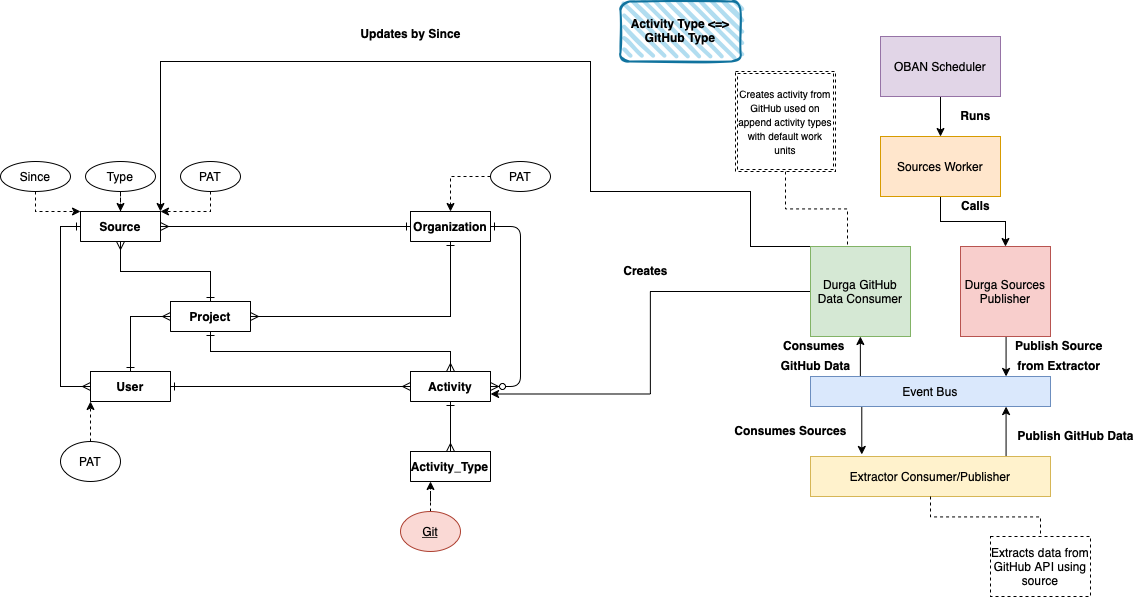
\includegraphics[scale=0.4]{Documentation/figures/diagram.png}  % largura percentual
	\caption{Entity-Relation and Workflow Diagram for Durga}
	\label{durga}
\end{figure}

\textbf{Key Components of the GitHub Data Extraction Life Cycle}

\begin{enumerate}
    \item \textit{Application Extractor}: The Application Extractor serves a vital function within the system, interacting directly with the GitHub API to fetch necessary data. It operates based on a publisher/consumer mechanism, subscribing to source events from the event bus and subsequently publishing GitHub data events. The interplay between subscription and publication establishes a fluid data pipeline from GitHub to Durga API app.
    \item  \textit{Durga GitHub Data Consumer}: This component acts as a subscriber to GitHub data events, transforming them into corresponding activity entries within the Durga API app. It identifies matches between the incoming GitHub data and valid activity types and associates them with the corresponding users through their GitHub handlers. One of its critical tasks is to update the \texttt{since} attribute on the sources, performed after successfully acknowledging the associated GitHub data for each source.
    \item \textit{Event Bus}: The Event Bus plays a critical role in the communication between the various components of the system. It is responsible for transmitting messages, which must adhere to a specific, enforced format to ensure the system accepts them. To facilitate the creation of new message types, a payload format must be defined. This task involves creating new \texttt{structs} for every accepted message type, ensuring data consistency, and enabling seamless communication across the system. 
    \item \textit{Sources Walker}: This worker already existed. It is responsible for checking the \texttt{since} attribute to ascertain the last update time for each source and then publishing a source event on the Event Bus. This regular crawling ensures that all sources are consistently monitored and any new activities are promptly identified and sent for further processing.
\end{enumerate}

The choice of an event bus architecture promotes fluid communication between applications that operate independently. These independent or 'decoupled' applications communicate through messages and remain agnostic to each other's internal workings. This design choice significantly simplifies scaling processes from a vertical and horizontal perspective. For example, if the workload related to data extraction experiences a surge - a likely scenario given that automated activity tracking constitutes a significant portion of Dharma Network's operations - multiple instances of the Extractor workers can be spawned effortlessly. These workers interconnected through the message bus, can efficiently distribute the workload among themselves and publish the results back to the same message bus.\newline

The Dharma Network team decided to adopt a decoupled architecture with a long-term vision in mind. By decoupling the applications, they could eliminate unnecessary dependencies and isolate potential faults, enhancing the system's overall resilience and flexibility. Furthermore, the modular approach fosters parallel development efforts, allowing teams to focus on a single component or service without being hindered by changes in others.\newline

In summary, the team's decision to choose a decoupled architecture was determined by the need for scalability, maintainability, resilience and development efficiency, which are vital for the ongoing success and growth of the Dharma Network.

\section{Development on Durga}

During the work on Durga, the main tasks that were assigned involved working within the Extractor and EventBus applications and creating a consumer within the Durga application. The work revolved around creating a complete lifecycle for data extraction from GitHub, beginning in Durga, proceeding through the Extractor, and then returning to Durga.

\subsection{Environment Variables}

The first official Dharma Network function to perform was to update the README.md. After the discovery of the crash of the program, it was necessary to update the README.md, so new developers could follow the rules. Information such as what Python version was compatible and the code lines that needed an update were added.\newline

Later, the implementation of environment variables was necessary. This feature had already been implemented on another project, as seen on section \ref{tentacat}, so the logic had already been taught.\newline

\textit{Environment variables} are variables set outside of the program and it's made up of a name/value pair. The whole point is to keep that information confidential.\newline

As for its implementation on Durga, they were set the following way: \newline

\begin{lstlisting}[language=erlang, caption={Environment Variables Configuration on .env.sample}]
# Remember to not leave any spaces between KEY and VALUE

 export JWT_SECRET=somekey

 export DEFAULT_PASS=anypassword

 # Username for the database
 export DATABASE_USERNAME=myusername

 # Password for the database
 export DATABASE_PASSWORD=mypassword

 # Name of the database
 export DATABASE_NAME=myapp_dev

 # Hostname for the database
 export DATABASE_HOST=host

 # Port for the database
 export DATABASE_PORT=port
\end{lstlisting}

\begin{lstlisting}[language=erlang, caption={Database configuration on dev.exs}]

 # Configure your database
 config :durga_api, DurgaApi.Repo,
   adapter: Ecto.Adapters.Postgres,
   username: System.get_env("DATABASE_USERNAME" || "database_name"),
   password: System.get_env("DATABASE_PASSWORD" || "database_password"),
   hostname: System.get_env("DATABASE_HOST" || "localhost"),
   database: System.get_env("DATABASE_NAME" || "developer_dev"),
   port: System.get_env("DATABASE_PORT" || "port_number"),
   stacktrace: true,
   show_sensitive_data_on_connection_error: true,
   pool_size: 15
\end{lstlisting}

This way, a developer can insert their information and it won't be stored when committing something on GitHub.\newline

\subsection{Extractor and Event Bus}

Once that was secured, it was time to work on what would be the most important feature developed and a key component of the entire project: the Extractor.\newline

The \textit{Extractor} followed the same lines of the Tentacat project (on section \ref{tentacat}). The solution was to develop a system that would extract the information requested by the user.\newline

This section already had some developed code, so the first interaction was not in terms of development, but of debugging. While debugging, it was clear to see that a significant portion of the provided code did not retrieve the expected information- or any information at all. Once the errors were specified, it was time to alter the existing code.\newline

Since the Extractor also had important information that was being stored on the code, environment variables were added. The Extractor needs information such as: \newline

\begin{lstlisting}[language=erlang, caption={Environment Variables Setup on extractor\_github.ex}]
token = System.get_env("GITHUB_TOKEN")
id = System.get_env("ID")
source_type = System.get_env("SOURCE_TYPE")
owner = System.get_env("GITHUB_OWNER")
user = System.get_env("GITHUB_USER")
repo = System.get_env("GITHUB_REPO")
since = System.get_env("SINCE_DATE")

\end{lstlisting}

As for the extraction of the GitHub information, it was made the following way:\newline

\begin{lstlisting}[language=erlang, caption={Commits extraction of extractor\_github.ex}]
@doc """
Shows every commit since given date, by all users
"""
def commits(token, id, org, repo, since) do
  client = Tentacat.Client.new(%{access_token: token})

  {_, commits, _} = Tentacat.Commits.filter(client, org, repo, %{
    since: since,
    per_page: 100
  })

  commits =
    commits
    |> Enum.filter(fn %{"parents" => parents} ->
      Enum.count_until(parents, 2) < 2
    end)
    |> Enum.map(&extract_commit/1)

  %{
    id: id,
    data: commits,
    source_type: :commits
  }
end
\end{lstlisting}

A client object is created using the \texttt{Tentacat} library (see \ref{tentacat}). The client is initialized with an access token.

It calls the \texttt{Tentacat.Commits.filter} function to retrieve a list of commits from a specified organization (\texttt{org}) and repository (\texttt{repo}). The \texttt{since} parameter specifies the starting date for the commits to retrieve, as the \texttt{per\_page} parameter limits the number of commits to be fetched to 100. If the filter wasn't selected, the default value would be 30. 

The result of this function call is a tuple containing three values, but the second value (commits) is of interest.

The \texttt{commits} list is then filtered using the texttt{Enum.filter function}. It checks each commit's "parents" field and keeps only those commits that have less than 2 parents. In other words, it \textit{filters out merge commits and keeps only the regular commits}.

The filtered commits are then transformed using the \texttt{Enum.map} function and a custom function \texttt{extract\_commit/1} is applied to each commit. The result is a new list of extracted commit data.

Finally, a map is constructed with the id, the filtered and extracted commits, and a \texttt{source\_type} field set to \texttt{:commits}. The map represents the result of the function.\newline


\begin{lstlisting}[language=erlang, caption={Pull requests extraction of extractor\_github.ex}]
@doc """
Shows every pull request since given date by a user (if specified) or all users (if null)
"""
def pull_requests(token, id, org, repo, since, user \\ nil) do
  client = Tentacat.Client.new(%{access_token: token})
  filters = %{state: "all", sort: "created", direction: "desc", creator: user, since: since}

  {_, pulls, _} = Tentacat.Issues.filter(client, org, repo, filters)

  pulls =
    Enum.filter(pulls, fn %{"user" => %{"login" => username}} ->
      is_nil(user) or username == user
    end)
    |> Enum.map(&extract_pull_request/1)

  %{
    id: id,
    data: pulls,
    source_type: :pull_requests
  }
end
\end{lstlisting}

 It creates a client using the \texttt{Tentacat.Client.new} function, passing the GitHub access token. Then, it defines the filters map containing the desired filter criteria, such as the state (can be open, closed or all), sort order (can be created, updated or comments), direction (can be ascending or descending), creator (the user that created the issue), and since date (timestamp in \texttt{ISO 8601} format: \textit{YYYY-MM-DDTHH:MM:SSZ}).\newline

 The \texttt{Tentacat.Issues.filter} function (see information on \ref{issue} to understand why we use \texttt{Issue} instead of \texttt{Pulls}) is invoked to retrieve the pull requests from the specified GitHub organization (\texttt{org}) and repository (\texttt{repo}) using the given filters. The result is stored in the pulls variable.\newline

The \texttt{Enum.filter} function is used to filter the pull requests based on the user parameter. If user is not \texttt{nil}, it only keeps the pull requests where the username matches the specified user. Otherwise, it keeps all pull requests. The filtered pull requests are then passed to the \texttt{Enum.map} function, which applies the \texttt{extract\_pull\_request/1} function to each pull request in order to extract the desired data.\newline

Finally, the function returns a map containing the id, data, and \texttt{source\_type} keys. The id is set to the provided id parameter, the data field holds the filtered and extracted pull requests stored in the pulls variable, and the \texttt{source\_type} is set to \texttt{:pull\_requests} to indicate the type of data retrieved.\newline

\begin{lstlisting}[language=erlang, caption={Reviews extraction of extractor\_github.ex}]
@doc """
Shows every review since given date and by given user (if specified) or all users (if null)
"""
def reviews(token, id, org, repo, since, user \\ nil) do
  client = Tentacat.Client.new(%{access_token: token})

  filters = %{sort: "created", direction: "desc", since: since}
  {_, comments, _} = Tentacat.Pulls.Comments.filter_all(client, org, repo, filters)

  reviews =
    Enum.filter(comments, fn %{"user" => %{"login" => username}} ->
      is_nil(user) or username == user
    end)
    |> Enum.map(&extract_review/1)

  %{
    id: id,
    data: reviews,
    source_type: :reviews
  }
end
\end{lstlisting}

It initializes the client using the \texttt{Tentacat.Client.new} function with the provided GitHub access token. The filters map is defined, specifying the sort order, direction, and since date for the comments.\newline

The \texttt{Tentacat.Pulls.Comments.filter\_all} function\footnote{This function was used because a review is considered if a pull request has two or more comments; if it only has one, it is considered a comment, so that information doesn't need to be retrieved.}\label{review} is called to retrieve all comments from the pull requests in the given GitHub organization (\texttt{org}) and repository (\texttt{repo}) based on the provided filters. The result is stored in the comments variable.\newline

The \texttt{Enum.filter} function is used to filter the comments based on the user parameter. If user is not \texttt{nil}, it only keeps the comments where the username matches the specified user. Otherwise, it keeps all comments. The filtered comments are then passed to the \texttt{Enum.map} function, which applies the \texttt{extract\_review/1} function to each comment in order to extract the desired data.\newline

Finally, the function returns a map containing the id, data, and \texttt{source\_type} keys. The id is set to the provided id parameter, the data field holds the filtered and extracted reviews stored in the reviews variable, and the \texttt{source\_type} is set to \texttt{:reviews} to indicate the type of data retrieved.\newline

\begin{lstlisting}[language=erlang, caption={Definition of private extraction functions of extractor\_github.ex}]
defp extract_commit(%{} = val) do
  val
end

defp extract_pull_request(%{} = val) do
  val
end

defp extract_review(%{} = val) do
  val
end
\end{lstlisting}

These extraction functions take a map as input and binds it to the variable val. The pattern \texttt{\%{} = val} matches any map. In this case, the functions don't perform any additional logic or transformation and simply return the input map val. They are used as helper functions.\newline

The EventBus was also implemented the following mode:\newline

\begin{lstlisting}[language=erlang, caption={Registry and Topics on event\_bus.ex}]
  @registry EventBus.Registry
  @topics [:source, :data]
\end{lstlisting}

\texttt{@registry} is a module attribute that holds the name of the registry used for event subscriptions. \texttt{@topics} is a module attribute that defines the list of supported topics.\newline

\begin{lstlisting}[language=erlang, caption={GenServer on event\_bus.ex}]
def start_link(_opts) do
  GenServer.start_link(__MODULE__, %{}, [{:name, __MODULE__}])
end
\end{lstlisting}

The \texttt{start\_link} function is the entry point for starting the \texttt{GenServer} process. It initializes the server state with an empty map \%{} and registers it with the name EventBus (the name of the module).\newline

\begin{lstlisting}[language=erlang, caption={Initialize state on event\_bus.ex}]
def init(state) do
  {:ok, state}
end
\end{lstlisting}

The \texttt{init} callback is called when the process is started and initializes the server state. In this code, it simply returns \texttt{\{:ok, state\}}.\newline

\begin{lstlisting}[language=erlang, caption={Subscribe to event topic on event\_bus.ex}, label={lst:unsub}]
def subscribe(key) do
  if Enum.member?(@topics, key) do
    {:ok, _} = Registry.register(EventBus.Registry, key, [])
    :ok
    case Registry.lookup(@registry, key) do
      [{pid, _}] ->
        {:ok, pid}
      [] ->
        {:ok, pid} = GenServer.start_link(__MODULE__, [], name: key)
        Registry.register(@registry, key, pid)
        {:ok, pid}
    end
  else
    :error
  end
end
\end{lstlisting}

The \texttt{subscribe} function is used to subscribe to a specific event topic. It takes a key parameter, which represents the topic to subscribe to. If the key is a member of the \texttt{@topics} list, it registers the topic in the \texttt{EventBus.Registry} and starts a new \texttt{GenServer} process for that topic if it doesn't already exist. It returns \texttt{:ok} if the subscription is successful, or \texttt{:error} if the key is not a supported topic.\newline

\begin{lstlisting}[language=erlang, caption={Unsubscribe to event topic on event\_bus.ex}]
def unsubscribe(key) do
  if Enum.member?(@topics, key) do
    Registry.unregister(@registry, key)
  else
    :error
  end
end
\end{lstlisting}

The \texttt{unsubscribe} function is used to unsubscribe from a specific event topic. It works the same way as the unsubscribe \ref{lst:unsub} does.\newline

\begin{lstlisting}[language=erlang, caption={Publish message on event\_bus.ex}]
def publish(:source, %EventBus.Messages.Source{} = payload) do
  publish_message(:source, payload)
end
def publish(:data, %EventBus.Messages.Data{} = payload) do
  publish_message(:data, payload)
end
\end{lstlisting}

The \texttt{publish} functions are used to publish messages to the event bus. They take a topic (\texttt{:source} or \texttt{:data}) and a payload as parameters. They call the private function \texttt{publish\_message} to handle the publishing of the message.\newline

\begin{lstlisting}[language=erlang, caption={Publish message's subscribers on event\_bus.ex}]
defp publish_message(key, payload) do
  Registry.dispatch(@registry, key, fn entries ->
    for {pid, _} <- entries, do: send(pid, {:publish, key, payload})
  end)
end
\end{lstlisting}

The \texttt{publish\_message} function retrieves the list of subscribers for the given key from the \texttt{EventBus.Registry} and sends the \texttt{\{:publish, key, payload\}} message to each subscriber process.\newline

\begin{lstlisting}[language=erlang, caption={Handle\_info on event\_bus.ex}]
def handle_info({:publish, key, payload}, state) do
  Logger.debug("Received message on topic #{inspect(key)} with payload: #{inspect(payload)}")
  case key do
    :source ->
      Logger.info("Received data from source: #{inspect(payload)}")
      {:noreply, state}
    :data ->
      Logger.info("Received data from data: #{inspect(payload)}")
      {:noreply, state}
    _ ->
      Logger.warn("Unsupported message: key=#{inspect(key)} payload=#{inspect(payload)}")
      {:noreply, state}
  end
end
\end{lstlisting}

The \texttt{handle\_info} callback is called when the server receives an asynchronous message. It handles messages of the form \texttt{\{:publish, key, payload\}}. It logs a debug message indicating the received message's topic and payload. Then, it matches the key to either \texttt{:source} or \texttt{:data} and logs an info message with the received payload. If the key doesn't match any known topic, it logs a warning message. Finally, it returns \texttt{\{:noreply, state\}} to indicate that no further action is required.\newline

Overall, the EventBus module provides a way to subscribe, unsubscribe and publish messages to different event topics, allowing communication between different processes in the application.\newline

When it comes to the connection with the Event Bus, the following was implemented:\newline

\begin{lstlisting}[language=erlang, caption={GenServer on extractor.ex}]
  def start_link(_opts) do
    GenServer.start_link(__MODULE__, %{}, [{:name, __MODULE__}])
  end
\end{lstlisting}

The \texttt{start\_link} function is the entry point for starting the \texttt{GenServer} process. It is responsible for initializing the server state and starting the process. In this case, it starts the Extractor process with an initial state of \%{} (an empty map) and registers it with the name Extractor (the name of the Module).\newline

\begin{lstlisting}[language=erlang, caption={Initialize state on extractor.ex}]
@impl true
def init(_state) do
  EventBus.subscribe(:source)
  {:ok, []}
end
\end{lstlisting}

The \texttt{init} callback is implemented as part of the \texttt{GenServer} behavior. It is called when the process is started and initializes the server state. In this code, it subscribes to the \texttt{:source} event on the EventBus and returns \texttt{\{:ok, []\}} as the initial state.\newline

\begin{lstlisting}[language=erlang, caption={Handle\_info for :source on extractor.ex}]
@impl true
def handle_info({:publish, :source, payload}, %{source: _source}) do
  GenServer.cast({:via, Registry, EventBus.Registry}, {:publish, :source, payload})

  {:noreply, state}
end
\end{lstlisting}

The \texttt{handle\_info} callback is called when the process receives an asynchronous message that is not handled by other specific message handlers. It handles the \texttt{\{:publish, :source, payload\}} message when the server state contains a key \texttt{:source}. It uses \texttt{GenServer.cast} to send a \texttt{\{:publish, :source, payload\}} message to the registered process via the Registry and EventBus.Registry. The return value \texttt{\{:noreply, state\}}indicates that no reply is sent to the sender of the message.\newline

\begin{lstlisting}[language=erlang, caption={Handle\_info for :data on extractor.ex}]
@impl true
def handle_info({:publish, :data, payload}, %{data: _data}) do
  GenServer.cast({:via, Registry, EventBus.Registry}, {:publish, :data, payload})

  {:noreply, state}
end
\end{lstlisting}

Similar to the previous \texttt{handle\_info} callback, this function handles the \texttt{\{:publish, :data, payload\}} message when the server state contains a key \texttt{:data}. It casts a \texttt{\{:publish, :data, payload\}} message to the registered process via the Registry and EventBus.Registry and returns \texttt{\{:noreply, state\}}.\newline

\begin{lstlisting}[language=erlang, caption={Handle\_info for key on extractor.ex}]
@impl true
def handle_info({:publish, key, payload}, state) do
  Logger.warn("Unsupported message: key=#{inspect(key)} payload=#{inspect(payload)}")

  {:noreply, state}
end
\end{lstlisting}

This is a fallback \texttt{handle\_info} callback that handles any other \texttt{\{:publish, key, payload\}} messages that are not explicitly matched by previous handlers. It logs a warning message indicating that an unsupported message was received, including the key and payload. It returns \texttt{\{:noreply, state\}}.\newline

This code handles incoming messages by either forwarding them to the registered process or logging a warning for unsupported messages.\newline

Amongst the development of this project, extensive testing and debugging were conducted to ensure its quality and reliability.\newline

\subsection{Publisher and Consumer}

The next step that wasn't fully completed was the creation of a publisher/consumer.\newline

A \textit{publisher} is a participant or entity responsible for generating and sending data or messages to a decentralized network or protocol.
The publisher is typically the source or originator of the information and initiates the process of sharing it with others.
They may publish data or messages through various means, such as posting on a decentralized platform, submitting transactions to a blockchain network or broadcasting messages to a peer-to-peer network.
The publisher may have specific intentions or objectives for sharing the data, such as disseminating news, providing updates or contributing to a decentralized application.\newline

As for the \textit{consumer}, it  is a participant or entity that receives and consumes data or messages from a decentralized network or protocol.
The consumer is interested in accessing or utilizing the information published by the publishers.
They retrieve data or messages from the network, typically by subscribing or requesting specific types of data they are interested in.
The consumer may process, analyze or use the received information for various purposes, such as displaying content to users, performing calculations or triggering specific actions.\newline

In decentralized systems, the publisher and consumer roles can be fulfilled by different participants or even automated processes. For example, in a decentralized messaging protocol, individual users can act as both publishers and consumers, sending and receiving messages to and from the network. Similarly, in a decentralized data marketplace, data providers act as publishers, offering their data for sale, while data buyers act as consumers, purchasing and utilizing the data.\newline

The objectives of this publisher are:

\begin{itemize}
    \item The publisher writes to the EventBus
    \item The publisher has its own API that can be called by other modules in the application
    \item Other modules can successfully publish extraction requests to Extractor.Github via the new publisher
    \item Extractor.Github successfully receives and processes the extraction requests sent by the new publisher.
\end{itemize}


As seen on figure \ref{durga}, Durga has an \texttt{Activity Type}, which will be fetched from GitHub by the consumer as follows:

\begin{lstlisting}[language=erlang, caption={Create Activity Type on activity\_consumer.ex}]
   defp create_commit_activities(<activity>) do
     activity_type = ActivityTypes.get_activity_type_by!(%{name: "github", description: "<description>"})
     [...]
\end{lstlisting}

\begin{lstlisting}[language=erlang, caption={Get Activity Type on activity\_types.ex}]
def get_activity_type_by!(params), do: Repo.get_by(ActivityType, params)
\end{lstlisting}

This way, it knows that the source is Github, since Dharma Network is planning on having multiple sources, like GitLab and others.\newline

The decoupled and modular architecture of the system was invaluable in this process. It allowed us to focus on specific system components, reducing dependencies on other parts and enhancing productivity. This practical experience provided a clear understanding of the benefits of such an architecture, further affirming the validity of the above design choices.\newline




 


